\documentclass[10pt,a4paper,titlepage,twoside]{report}
\usepackage{polski}
\usepackage[utf8]{inputenc}
\usepackage[T1]{fontenc}
\usepackage{graphicx}
\usepackage{sidecap}
\usepackage{wrapfig}
\usepackage{makecell}
\usepackage{subfig}
\usepackage{enumerate}
\usepackage{amssymb}
\usepackage{geometry}
\usepackage{pgfpict2e}
\usepackage{tikz}
\usepackage{wrapfig}
\usepackage{floatflt}
\usepackage{multirow}
\usepackage{comment}
\usepackage{array}
\usepackage{pbox}
\usepackage{setspace}
\usepackage{helvet}
\renewcommand{\familydefault}{\sfdefault}
\usepackage{chngcntr}
\usepackage{amsmath}
\usepackage{xcolor,colortbl}
\usepackage{cite}
\counterwithin{figure}{chapter}
\newcommand{\done}{\cellcolor{teal}done}

\begin{document}


\newgeometry{tmargin=2.5cm, bmargin=2.5cm, lmargin=3.5cm, rmargin=2.5cm}
\setlength{\parindent}{1.25cm}

%\justify


\begin{titlepage}
  \begin{center}


\begin{center}
\begin{tabular}{l l r}
 	
\includegraphics[scale=0.26]{pics/pg_weti.png} & \hspace*{5cm} &  
\includegraphics[width=0.13\textwidth]{pics/eti.png}\\
\end{tabular}
\end{center}

\vspace*{0.5cm}

\begin{flushleft}

	Imię i nazwisko studenta: Michał Żyłowski\\
	\vspace*{0.1cm}
	Nr albumu: 137448\\
	\vspace*{0.1cm}
	Studia drugiego stopnia\\
	\vspace*{0.1cm}
	Forma studiów: stacjonarne\\
	\vspace*{0.1cm}
	Kierunek studiów: Informatyka\\
	\vspace*{0.1cm}
	Specjalność/profil: TODO!!!\\


\end{flushleft}

\vspace*{1.8cm}

\begin{flushleft}
{ \large {\bf{PRACA DYPLOMOWA MAGISTERSKA}}  }
\end{flushleft}

\vspace*{1cm}

\begin{flushleft}
Tytuł pracy w języku polskim: TODO\\
\vspace*{0.4cm}
Tytuł pracy w języku angielskim: TODO\\
\end{flushleft}

\vspace*{1.5cm}
\renewcommand{\arraystretch}{1.5}
\begin{tabular}{|l  |l|}
	\hline
 	\multicolumn{2}{|l|} {Potwierdzenie przyjęcia pracy } \\
	\hline
	Opiekun pracy & Kierownik Katedry/Zakładu \hspace*{2cm} \\
	&\\
	\small \textit{podpis} & \small  \textit{podpis}\\
	\hline
	dr inż. Jerzy Demkowicz & dr hab. inż. Marek Moszyński, prof. nadzw. PG \hspace*{2cm} \\
	&\\
    \hline

\end{tabular}

\vspace*{2.5cm}

\begin{flushleft}
	Data oddania pracy do dziekanatu: \\
\end{flushleft}


 \end{center}

\end{titlepage}


\newgeometry{top=2.5cm, bottom=2.5cm, left=2.5cm, right=3.5cm}

\newpage
\thispagestyle {empty}

\begin{center}
\begin{tabular}{l l r}
 	
\includegraphics[scale=0.26]{pics/pg_weti.png} & \hspace*{5cm} &  
\includegraphics[width=0.13\textwidth]{pics/eti.png}\\
\end{tabular}
\end{center}

\vspace*{0.1cm}

\begin{flushleft}
	\large{\bf{OŚWIADCZENIE}}\\
\end{flushleft}

\vspace*{0.1cm}

\begin{flushleft}

	Imię i nazwisko: Michał Żyłowski\\
	\vspace*{0.1cm}
	Data i miejsce urodzenia:  XX.XX.XXXTODO, Toruń\\
	\vspace*{0.1cm}
	Nr albumu: 137448\\
	\vspace*{0.1cm}
	Wydział: Wydział Elektroniki, Telekomunikacji i Informatyki\\
	\vspace*{0.1cm}
	Kierunek: informatyka\\
	\vspace*{0.1cm}
	Poziom studiów: II stopnia - magisterskie\\
	\vspace*{0.1cm}
	Forma studiów: stacjonarne\\

\end{flushleft}

\vspace*{0.5mm}

Ja, niżej podpisany(a), wyrażam zgodę/nie wyrażam zgody* na korzystanie z mojej pracy dyplomowej zatytułowanej: Ewolucyjny wieloagentowy system bezzałogowych łodzi monitorujących akweny morskie
do celów naukowych lub dydaktycznych. \footnote{ Zarządzenie Rektora Politechniki Gdańskiej nr 34/2009 z 9 listopada 2009 r., załącznik nr 8 do instrukcji archiwalnej PG.}\\
Gdańsk, dnia  ........................  \hspace{5cm}
\begin{tabular}{c}
	\\
	  .............................\\
	\small \textit{podpis studenta}
\end{tabular}

\vspace*{0.5mm}

Świadomy(a) odpowiedzialności karnej z tytułu naruszenia przepisów ustawy z dnia 4 lutego 1994 r. o prawie autorskim i prawach pokrewnych (Dz. U. z 2006 r., nr 90, poz. 631) i konsekwencji dyscyplinarnych określonych w ustawie Prawo o szkolnictwie wyższym (Dz. U. z 2012 r., poz. 572 z późn. zm.),\footnote{ Ustawa z dnia 27 lipca 2005 r. Prawo o szkolnictwie wyższym:\\ Art. 214 ustęp 4. W razie podejrzenia popełnienia przez studenta czynu podlegającego na przypisaniu sobie autorstwa istotnego fragmentu lub innych elementów cudzego utworu rektor niezwłocznie poleca przeprowadzenie postępowania wyjaśniającego.\\Art. 214 ustęp 6. Jeżeli w wyniku postępowania wyjaśniającego zebrany materiał potwierdza popełnienie czynu, o którym mowa w ust. 4, rektor wstrzymuje postępowanie o nadanie tytułu zawodowego do czasu wydania orzeczenia przez komisję dyscyplinarną oraz składa zawiadomienie o popełnieniu przestępstwa.} a także odpowiedzialności cywilno-prawnej oświadczam, że przedkładana praca dyplomowa została opracowana przeze mnie samodzielnie.\\
\newline
Niniejszy projekt dyplomowy nie był wcześniej podstawą żadnej innej urzędowej procedury związanej z nadaniem tytułu zawodowego.\\
\newline
Wszystkie informacje umieszczone w ww. projekcie dyplomowym, uzyskane ze źródeł pisanych i elektronicznych, zostały udokumentowane w wykazie literatury odpowiednimi odnośnikami zgodnie z art. 34 ustawy o prawie autorskim i prawach pokrewnych.\\
\newline
Potwierdzam zgodność niniejszej wersji projektu dyplomowego z załączoną wersją elektroniczną\\

\noindent Gdańsk, dnia  ........................  \hspace{5cm}
\begin{tabular}{c}
	\\
	  .............................\\
	\small \textit{podpis studenta}
\end{tabular}

Upoważniam Politechnikę Gdańską do umieszczenia ww. pracy dyplomowej w wersji elektronicznej w otwartym, cyfrowym repozytorium instytucjonalnym Politechniki Gdańskiej oraz poddawania jej procesom weryfikacji i ochrony przed przywłaszczaniem jej autorstwa.\\
\newline
Gdańsk, dnia  ........................  \hspace{5cm}
\begin{tabular}{c}
	\\
	  .............................\\
	\small \textit{podpis studenta}
\end{tabular}





*) niepotrzebne skreślić




\newpage
\newgeometry{top=2.5cm, bottom=2.5cm, left=3.5cm, right=2.5cm}
\setcounter{page}{1}
\onehalfspacing

\section*{Streszczenie}
\addcontentsline{toc}{section}{Streszczenie}
\indent  TODO\\

\noindent \textbf{Słowa kluczowe:} TODO

\newpage
\section*{Abstract}
\addcontentsline{toc}{section}{Abstract}

TODO\\
\newline
\textbf{Keywords:} TODO


\newpage
\newgeometry{top=2.5cm, bottom=2.5cm, left=2.5cm, right=3.5cm}

\tableofcontents


\newpage
\newgeometry{top=2.5cm, bottom=2.5cm, left=2.5cm, right=3.5cm}
\section*{Wykaz ważniejszych oznaczeń i skrótów}
\addcontentsline{toc}{section}{Wykaz ważniejszych oznaczeń i skrótów}



DC - (ang. \textit{Data Center}) Centrum Danych\\
\newline


\newpage
\newgeometry{top=2.5cm, bottom=2.5cm, left=2.5cm, right=3.5cm}

\onehalfspacing

\chapter{Wstęp i cel pracy}
\section{Charakterystyka klastrów obliczeniowych}
\indent \indent Na przestrzeni lat znacząco wzrosła liczba użytkowników Internetu\cite{ad1}. Obecnie utrzymywanie kilku stron internetowych, odwiedzanych każdego dnia przez wielu użytkowników jest znacznie trudniejsze niż kiedyś\cite{ad1}. Liczba treści w Internecie sprawia, że bazy danych rosną w zastraszającym tempie, a bardziej skomplikowane zapytania konsumują duże ilości zasobów na maszynach. Aby walczyć z tymi problemami można optymalizować kod, zwiększać liczbę dostępnych zasobów - dokładać pamięci operacyjnej, stosować szybsze dyski czy używać procesorów z większą ilością rdzeni, lub wyższym taktowaniem. Mimo takich działań administratorzy serwerów niebawem znajdą się w sytuacji, w której konieczne będzie użycie kolejnej maszyny, aby poradzić sobie z obsługą generowanego przez użytkowników ruch\cite{ad2}. Stworzy to wiele problemów z którymi administrator będzie musiał sobie poradzić: współdzielenie oraz synchronizowanie bazy danych między maszynami, rozkładanie obciążenia między maszyny i wiele innych\cite{ad2}.

Jeśli strona internetowa osiągnie prawdziwy sukces i obsługa będzie wymagała kolejnych serwerów, administrator zetknie się z problemem monitorowania maszyn, wydzielenia dysków czy tworzeniem kopii zapasowych. Wiele serwerów to też problem utylizacji zasobów. Konieczne jest takie rozłożenie zadań na naszym klastrze by zmaksymalizować użycie zasobów na poszczególnych serwerach - każda nieużywana pamięć to strata pieniędzy i energii\cite{ad3}.

\begin{figure}[ht!]
	\centering
	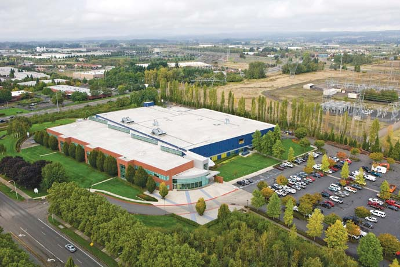
\includegraphics[scale=0.7]{pics/Selection_615.png}
	\caption{Centrum danych Facebooka w Oregonie, grafika pochodzi ze strony http://siteselection.com/}
	\label{facebook_dc}
\end{figure}


Dla przykładu firma Facebook, na samym początku swojego istnienia obsługiwała cały ruch za pomocą wyłącznie jednej maszyny\cite{ad4}. Było to w czasach gdy serwis ten nie wspierał jeszcze wrzucania obrazków, czy filmów przez użytkowników. W kwietniu 2008 roku centrum danych Facebooka liczyło już 10 tysięcy maszyn, by dwa lata później osiągnąć już 60 tysięcy. Obecnie korporacja nie zdradza informacji ile serwerów utrzymuje, ale rozmiar ich farmy serwerów w Oregonie (Rys. \ref{facebook_dc}), mówi sam za siebie - 307 tysięcy metrów kwadratowych\cite{ad5}.

Powyższy problem dotyczy tylko jednego typu zadania, czyli hostingu wymagającego web serwisu. Współczesny świat współtworzony jest przez wiele rodzajów zadań: konwersja wideo, obliczanie skomplikowanych matematycznych równań, przechowywanie i prezentowanie map i wiele innych. Poszczególne rodzaje zadań często interferują ze sobą. Ich umieszczanie na jednym serwerze może doprowadzić do walki o zasoby między procesami. Pojawia się więc problemem utylizacji serwerowni, czyli rozłożenia zadań tak by nie kolidowały ze sobą, ale także aby zminimalizować ilość nieużywanych zasobów\cite{ad5}.

\subsection{Podział klastrów obliczeniowych}\indent \indent Ze względu na pełnione funkcje, możemy wyróżnić następujące rodzaje klastrów obliczeniowych\cite{ad6}.

\begin{itemize}
	\item \textbf{Klastry wydajnościowe (ang. \textit{High Performance Computing Clusters})} - moc obliczeniowa jest wykorzystywana do przeprowadzania bardzo skomplikowanych obliczeń matematycznych, trwających nawet wiele miesięcy. Służą do przetwarzania jednego rodzaju danych (np. porównywanie kodów DNA, przygotowywanie markerów rakowych itp.).
	\item \textbf{Klastry równoważące obciążenie (ang. \textit{Load Balancing Clusters})} - ich główne zadanie polega na równoważnym dystrybuowaniu obciążenia między poszczególne serwery  (węzły klastra). Tego typu klaster instaluje się w systemach, w których bardzo istotny jest czas reakcji na zadanie klienta. Load balancer przesyła nadchodzące żądania obsługi do węzłów, które posiadają niezagospodarowane w danej chwili moce obliczeniowe, odciążając tym samym węzły, które są w danym momencie bardzo obciążone i zbyt wolno odpowiadają by obsłużyć kierowane do serwera żądania w wymaganym czasie. Przykładowe zastosowanie takiego klastra to hosting stron internetowych, czyli udostępnianie mniej lub bardziej złożonych aplikacji internetowych klientowi końcowemu. Często wymaga to zainstalowania na klastrze systemów bazodanowych oraz interpreterów specyficznych dla technologii w której wytworzony jest web serwis.
	\item \textbf{Klastry niezawodnościowe (ang. \textit{High Availability Clusters})} - klastry o wysokiej dostępności. Klastry tego typu nie zwiększają wydajności serwisów, a mają jedynie eliminować tzw. pojedynczy punkt awarii (ang. Single Point of Failure) - w razie uszkodzenia jednego z serwerów jego zadania są, w sposób niewidoczny dla użytkowników, przejmowane przez inny węzeł klastra.
\end{itemize}

\subsection{Podział chmur ze względu na zainstalowane oprogramowanie}\indent \indent Klaster obliczeniowych na którym zainstalowano i skonfigurowano odpowiednie oprogramowanie będziemy nazywać chmurą obliczeniową. W zależności od zainstalowanego na klastrze oprogramowania, możemy wyróżnić następujące rodzaje chmur\cite{ad6}:
\begin{itemize}
	\item \textbf{Infrastructure as a Service (IaaS)} - zasoby serwerów klastra są wydzielane i odizolowywane od siebie a następnie przedstawiane są użytkownikowi końcowemu jako niezależne serwery. Ten rodzaj chmur obliczeniowych mogą wykorzystywać firmy, które chcą sprzedawać niewielkie serwery swoim klientom. Model tej usługi polega na dostarczaniu klientowi infrastruktury informatycznej czyli sprzętu, oprogramowania oraz serwisowania. Klient wykupuje na przykład konkretną liczbę serwerów, przestrzeni dyskowej, lub określony zasób pamięci i mocy obliczeniowej. Nie oznacza to jednak, że sprzęt fizycznie zostanie zainstalowany w siedzibie klienta\cite{ad7}. W tym modelu zdarza się, że klient dostarcza usługodawcy własne oprogramowanie do zainstalowania na wynajmowanym sprzęcie.
	\item \textbf{Platform as a Service (PaaS)} - w tym modelu sprzedaż gotowego, często dostosowanego do potrzeb użytkownika, kompletu aplikacji nie wiąże się z koniecznością zakupu sprzętu ani instalacją oprogramowania. Wszystkie potrzebne programy znajdują się na serwerach dostawcy\cite{ad9}. Klient po swojej stronie ma dostęp do interfejsu (na ogół w postaci ujednoliconego środowiska pracy) poprzez program – klienta. np. przeglądarkę internetową. W tym modelu usługi najczęściej dostępne są dla użytkownika z dowolnego połączonego z Internetem komputera.
	\item \textbf{Software as a Service (SaaS)} - aplikacja jest przechowywana i wykonywana na komputerach dostawcy usługi i jest udostępniana użytkownikom przez Internet. Eliminuje to potrzebę instalacji i uruchamiania programu na komputerze klienta. W tym modelu użytkownik oddaje kontrolę nad oprogramowaniem dostawcy i obowiązek zapewnienia ciągłości jego działania. Istotą biznesową oprogramowania w modelu SaaS, decydującą o jej rosnącej popularności jest to, że użytkownik kupuje działające rozwiązanie o określonej funkcjonalności bez konieczności wchodzenia w zagadnienia związane z infrastrukturą informatyczną oraz zapleczem technicznym. W wielu przypadkach SaaS umożliwia dostęp do najnowszych technologii informatycznych bez długotrwałych wdrożeń i dużych inwestycji\cite{ad8}.
	\item \textbf{Data as a Service (DaaS)} - polega na udostępnieniu użytkownikowi przestrzeni dyskowej, którą może wykorzystać do przechowania plików\cite{ad10}, np. zdjęć, muzyki, filmów itd. Chmury tego typu oferują interfejs (np. w postaci web serwisu), który umożliwia łatwą komunikację i zarządzanie utrzymywanymi plikami. Interfejsy w takiej chmurze pozwalają na łatwe dzielenie się danymi z innymi użytkownikami, np. przy pomocy odpowiednich linków.
	\item \textbf{Storage as a Service (STaaS)} - polega na udostępnieniu użytkownikowi przestrzeni dyskowej, która może być przez niego dowolnie wykorzystana. W tym modelu klient końcowy otrzymuje bezpośredni dostęp do urządzeń lub bloków pamięci i to po jego stronie leży zaprojektowanie mechanizmu, który będzie z tych udostępnionych zasobów korzystał\cite{ad10}. Jest to główna różnica między chmurą typu DaaS, w której to, użytkownik ma przygotowany interfejs, również uruchomiony w chmurze.
	\item \textbf{Security as a Service (SecaaS)} - podejście polegające na uruchamianiu oprogramowania antywirusowego w chmurze. Klient takiej chmury otrzymuje wszystkie funkcje programów antywirusowych (skanowanie plików, heurystyka itd.) bez konieczności uruchamiania antywirusa na swoim sprzęcie. Ze względu na ogromne ilości danych przesyłanych między chmurą z antywirusem, a końcowym użytkownikiem, tego typu rozwiązania mogą mieć głównie zastosowania w lokalnych serwerowniach (wysokie przepustowości między maszynami w jednym centrum danych).
\end{itemize}
\subsection{Podział chmur ze względu na lokalizację infrastruktury technicznej}
\begin{itemize}
	\item \textbf{Chmura prywatna (ang. \textit{Private Cloud})} - rozwiązanie polega na zakupieniu przez dany ośrodek fizycznych serwerów, podłączeniem ich w serwerowni oraz zainstalowaniem całego oprogramowania od zera\cite{ad10}. Chmura prywatna to inwestycja, która wymaga dużego wkładu początkowego (zakup serwerów), oraz ponoszenia ciągłych kosztów związanych z zasilaniem i chłodzeniem uruchomionych serwerów. Nie bez znaczenia pozostaje koszt związany z zatrudnieniem kadry i administratorów odpowiedzialnych za utrzymanie serwerów jak i całego centrum danych. Chmura prywatna daje użytkownikowi końcowemu pełną swobodę i możliwość całkowitego ingerowania w swoją infrastrukturę. Odpowiednio przygotowana polityka bezpieczeństwa będzie dawała pewność, że nikt postronny nie ma dostępu do danych. Własna serwerownia to też szybsze prędkości i od uniezależnienie się od wolniej działającej sieci Internet\cite{ad11}.
	\item \textbf{Chmura publiczna (ang. \textit{Public Cloud})} - rozwiązanie polega na wykupieniu u wybranego dostawcy (ang. providera) odpowiedniego rozwiązania. W tym podejściu cała infrastruktura z której korzystamy znajduje się u dostawcy, zaś klient otrzymuje do niej dostęp poprzez sieć Internet i odpowiednie protokoły dostępu\cite{ad12}. W rozwiązaniach typu Public Cloud wszystkie dane są trzymane na infrastrukturze dostawcy, a co za tym idzie, klient chmury nie ma nad nimi pełnej kontroli. Jest to jeden z głównych powodów, dla których firmy szczególnie chroniące swoje dane, bądź pracujące nad rozwiązaniami poufnymi niechętnie korzystają z tego rozwiązania\cite{ad11}. Na rynku chmur obliczeniowych trwa niekończąca się dyskusja \cite{ad13}, na temat opłacalności chmur publicznych w stosunku do prywatnych. Używanie chmury publicznej generuje koszty, które ponoszone są przez klienta (comiesięczne rachunki). Chmury publiczne dostosowują się do obciążenia i wymagań użytkownika, tzn. jeśli dotychczasowe zasoby są niewystarczające by obsłużyć ruch, zasoby klienta są automatycznie powiększane z jednoczesnym podwyższeniem kwoty do zapłacenia w kolejnym okresie rozliczeniowym. W ostatecznym rozrachunku, po kilku latach używania i opłacania chmury publicznej może się okazać, że całkowite wydatki znacznie przewyższyły jednorazowy wydatek, który trzeba by ponieść by zakupić na własny użytek chmurę prywatną. Warto w tym miejscu wspomnieć o ważnej zalecie chmury publicznej, tj. możliwość kolokacji zasobów i federowania uruchomionych usług. Dostawcy chmur publicznych często posiadają wiele centrów danych\cite{ad11}. Zwiększa to bezpieczeństwo naszych danych – nawet atak na jakiś kraj i całkowity jego paraliż nie spowoduje wyłączenia naszych usług, gdyż będzie możliwe ich natychmiastowe uruchomienie w centrum danych po drugiej stronie globu. Tak rozwiązanie umożliwia również odpowiednie dzielenie obciążenia naszych usług o ile tylko są one do tego przystosowane. Użytkownicy końcowi usługi w chmurze, łączący się np. z USA skorzystają z centrów danych rozlokowanych w Ameryce Północnej, zaś klient z Europy połączy się z odpowiednim dla niego centrum danych ze starego kontynentu\cite{ad11}.
	\item \textbf{Chmury hybrydowe (ang. \textit{Hybrid Cloud})} - rozwiązanie polegające na połączeniu chmur publicznych i chmur prywatnych\cite{ad13}. Zazwyczaj celem jest uwypuklenie zalet obu tych rozwiązań – tj. przechowywanie danych w chmurze prywatnej, zaś dokonywanie obliczeń, bądź serwowanie treści web serwisu po stronie chmury publicznej. Innym często spotykanym rozwiązaniem jest uruchamianie zadań na chmurze prywatnej, zaś chmura publiczna jest używana do przechowywania kopii bezpieczeństwa\cite{ad13}.
\end{itemize}

\subsection{Podział klastrów obliczeniowych}\indent \indent Uruchamianie aplikacji na chmurach obliczeniowych stwarza wiele problemów, które nie były spotkane przy klasycznym podejściu \cite{ad14}. Mowa tu między innymi o:
\begin{itemize}
	\item Napisaniu aplikacji w taki sposób by działała na chmurze.
	\item Aplikacja powinna współpracować z innymi uruchomionymi instancjami.
	\item Odpowiednim odizolowaniu od siebie zadań na poszczególnych serwerach.
	\item Optymalnym podzieleniu zadań pomiędzy dostępne zasoby.
	\item Zaprojektowaniu architektury sieciowej w serwerowni, tak aby była odporna na ataki z zewnątrz oraz możliwie optymalizowała ruch pomiędzy maszynami.
	\item Osiągnięciu wysokiego poziomu utylizacji całego centrum danych.
\end{itemize}

\section{Cel oraz zakres projektu}
\indent \indent Projekt realizowany jest w ramach pracy dyplomowo-magisterskiej na semestrze trzecim studiów stacjonarnych II stopnia na kierunku “Informatyka” wydziału Elektroniki, Informatykii Telekomunikacji Politechniki Gdańskiej.

W powyższym podrozdziale wypisałem kilka podstawowych problemów dotyczących chmur obliczeniowych. W niniejszej pracy chciałbym szczególnie skupić się na jednym z nich, mianowicie utylizacji centrum danych. Wykładowca z uniwersytetu Stanford, Christos Kozyrakis w jednej ze swoich publikacji[3] udowadnia tezę, która mówi o bardzo niskim poziomie utylizacji całego centrum danych. Według jego dowodów poziom utylizacji w typowym centrum danych to około 20 procent. Doktor Christos wskazuje, jak drogie jest utrzymywanie centrum danych (chłodzenie, zasilanie) w stosunku do poziomu utylizacji jaką właściciel serwerowni jest w stanie utrzymać. W pracy wspiera się pogląd, że zamiast inwestować w kolejne serwery, wcześniej należy podjąć próby zoptymalizowania pracy całego centrum danych. Wg. autora pracy, należy przyjrzeć się dwóm kwestiom: odpowiedniego odizolowania zadań (tak aby nie interferowały one między sobą) oraz optymalnego i odpowiedzialnego rozdzielenia je na poszczególne zasoby, którymi dysponuje administrator.

Moja praca magisterska dotyczy analizy narzędzia Mesos i jego frameworków, pod kątem zarządzania zasobami w centrum danych, ze szczególnym zwróceniem uwagi na zwiększanie poziomu utylizacji całej serwerowni. W pracy dokonam przeglądu kilku istniejących na rynku frameworków i przeprowadzę analizę w oparciu o dokonane w ramach projektu magisterskiego pomiary. Krótko opiszę i zbadam kilka mechanizmów izolacji wykorzystywanych współcześnie.

Rozwiązanie Mesos wybrałem ze względu na jego stabilność i wysoki poziom adopcji na rynku chmur obliczeniowych. Mesos’a wykorzystuje wiele firm [17], np.: Allegro, Twitter, eBay czy Samsung. Więcej informacji na temat rozwiązań konkurencyjnych opiszę w dalszej części pracy.

Całe oprogramowane, które zostało przenalizowane bądź opisane w tej pracy było oprogramowaniem otwartym i darmowym. Również wszystkie produkty powstałe wraz z tą pracą są udostępnione na takiej właśnie licencji.

Mesos jest rozwiązaniem rozpowszechnianym na licencji Apache 2.0. Od lat produktem zajmuje się firma Mesosphere. Firma ta przygotowała grupę rozwiązań związanych z chmurami obliczeniowymi oraz silnie włączyła się w rozwijanie Mesosa. Dzięki wsparciu tej firmy udało się wydać wersję 1.0 (przeskok z wersji 0.26). Przyłączenie się Mesosphery do rozwoju Mesosa przyniosło też minusy. Najbardziej znaczącym z nich jest spadek zainteresowania „czystym” Mesosem na rzecz produktu Mesosphery „DC/OS” – Data Center Operating System. Narzędzie prócz samego Mesosa zawiera zaawansowany instalator, wsparcie dla sklastrowanego systemu przechowywania danych, zunifikowany dostęp do logów, oraz rozbudowanego klienta CLI. Rozwiązanie DC/OS dostępne jest w dwóch wersjach - darmowej oraz skierowanej do klientów biznesowych. Wykupienie rozwiązania biznesowego pozwoli na korzystanie z pomocy technicznej, oraz zaawansowanych mechanizmów dotyczących bezpieczeństwa na uruchomionym klastrze.

Rozwój platformy sprawił, że w literaturze i Internecie brakuje informacji o samym Mesosie. Z tego powodu wraz z powstaniem tej pracy przygotowany został produkt Mesos-dockerized – udostępniony na repozytorium na github.com. Mój produkt umożliwia zestawienie najnowszej stabilnej wersji Mesosa w kontenerach na swoim klastrze.

Drugim produktem, który powstał wraz z tą pracą jest proste narzędzie pozwalające na uruchamianie zadań poprzez poszczególne frameworki Mesosa. Również udostępniony jest on na githubie, jako wolne oprogramowanie udostępnione na licencji MIT.

Utworzenie tych produktów, pozwoliło mi na zestawienie klastra na infrastrukturze otrzymanej od prowadzącego, uruchomienie tam chmury obliczeniowej za pomocą Mesosa oraz wykonanie testów i pomiarów, które opisane są w dalszej części pracy. Opierając się o nie przygotowałem podsumowanie, które odpowiada na postawione w tej pracy pytanie: „Czy Mesos pozwala zwiększyć poziom utylizacji centrum danych, w którym jest uruchomiony”.

Praca zawiera opis poszczególnych frameworków, szczegółowy opis architektury Mesos’a, wewnętrznych mechanizmów narzędzia, sposobów zestawiania go na klastrze, oraz instrukcje uruchamiania zadań. W kilku zdaniach poruszone zostały rozwiązania konkurencyjne, a problem izolacji został dokładnie sprawdzony również w innym, konkurencyjnym rozwiązaniu.

\section{Wirtualizacja}
\indent \indent Wirtualizacja – użycie oprogramowania i utworzenie kolejnej warstwy abstrakcji w celu stworzenia iluzji posiadania pewnych zasobów. Zasoby te będą zwirtualizowane, tzn. ich istnienie będzie programowo symulowane, bądź też system operacyjny za pomocą odpowiednich mechanizmów wydzieli część fizycznie istniejących zasobów i pozwoli maszynie wirtualnej ich używać[14].

Maszyna wirtualna – wydzielona przestrzeń komputera hosta, która zostaje przedstawiona jako nowe urządzenie. Użytkownik maszyny wirtualnej może uruchomić na maszynie wirtualnej zadany system operacyjny, który będzie korzystał ze zwirtualizowanych wcześniej zasobów[14].

\subsection{Kryteria wirtualizacji}\indent \indent Kryteria wirtualizacji zostały przedstawione w 1976 roku przez dwóch naukowców – Geralda Popka oraz Roberta Goldberga. Są to[14]:
\begin{itemize}
	\item Zasada odpowiedniości – aplikacja działająca na maszynie wirtualnej musi zachowywać się w dokładnie taki sam sposób, jak na rzeczywistym sprzęcie.
Gdy aplikacja łamie to kryterium, przyczyną może być brak wirtualizacji wymaganych mechanizmów, bądź błędne zwirtualizowanie, któregoś z nich. Przykładowo: Trudnym problem jest wydzielanie fragmentu karty graficznej, bądź jej wirtualizowanie. Gdy użytkownik spróbuje uruchomić wymagającą aplikację graficzną na maszynie wirtualnej, na której nie jest dostępna zwirtualizowana karta graficzna, całość obliczeń graficznych przenoszona jest na wirtualne procesory, a co za tym idzie, dochodzi do ogromnego spadku wydajności.
	\item Kontrola zasobów – wirtualna maszyna musi w pełni kontrolować wszystkie zasoby, które są wirtualizowane. Wirtualizator powinien na samym początku tworzenia maszyny, zarezerwować wszelkie potrzebne zasoby, oraz sprawować nad nimi kontrolę aż do wyłączenia danej maszyny. Taka rezerwacja i kontrola jest potrzebna, ze względu na wywłaszczenia których dokonuje host maszyny wirtualnej. Raz przypisane zasoby, powinny należeć do maszyny wirtualnej, aż do jej wyłączenia.
	\item Wydajność – większa część instrukcji musi być wykonywana bez udziału maszyny wirtualnej.
To kryterium jest kluczowe dla pojęcia wirtualizacji. Instrukcje aplikacji powinny być podzielone pomiędzy zwirtualizowane zasoby, a zasoby fizyczne (hosta). Aby uzyskać zysk wydajnościowy należy możliwie wiele instrukcji wykonać bez udziału maszyny wirtualnej. Jednakże instrukcje muszą być rozdzielne w taki sposób by odizolować się od innych aplikacji na komputerze hosta – wykonanie powodujące błędy na maszynie wirtualnej nie wpływa na aplikacje na innych maszynach wirtualnych. Opisany tutaj podział jest największym wyzwaniem przy tworzeniu wirtualizatorów. Od zastosowanych mechanizmów podziału zależy jaki poziom izolacji zostanie osiągnięty. Im lepsza izolacja zasobów, tym lepsza jakoś wirtualizacji[18].
\end{itemize}

\subsection{Rodzaje wirtualizacji}\indent \indent Pojęcie wirtualizacji jako abstrakcji zasobów jest niezwykle szerokie i obejmuje wiele rozwiązań o zupełnie różnych zastosowaniach. Dlatego oddzielnie rozważę kilka gałęzi technologicznych, które składają się na to zagadnienie [14][19]:

\begin{itemize}
	\item Emulacja (pełna wirtualizacja z dynamiczną rekompilacją) - program emulujący zazwyczaj udaje wyłącznie inny rodzaj sprzętu komputerowego bez jakiegokolwiek oprogramowania, czego efektem jest konieczność instalacji systemu operacyjnego na emulatorze. Emulatory pozwalają używać oprogramowania, do którego sprzęt może fizycznie już nie istnieje, bądź nie jest produkowany.
	\item Wirtualizacja natywna (pełna wirtualizacja) - umożliwia uruchamianie systemu operacyjnego kompatybilnego z posiadanym systemem komputerowym i dokonuje wirtualizacji tylko części wywołań, potrzebnych do izolacji oprogramowania. Cała reszta jest przetwarzana przez fizyczny sprzęt, celem zwiększania wydajności wirtualizacji. Zwykle polega to na stworzeniu maszyny wirtualnej przechwytującej wszystkie wywołania, a następnie przekazywaniu wybranych instrukcji do systemu komputerowego. Przekazuje się przede wszystkim instrukcje wejścia/wyjścia i obsługi sieci.
	\item Parawirtualizacja (hipernadzorca) - w tym przypadku oprogramowanie wirtualizujące nie tworzy iluzji sprzętu, a jedynie dostarcza programowe API, z którego mogą korzystać odpowiednio zmodyfikowane systemy operacyjne. Jest to alternatywa szczególnie dla architektury x86, która jest trudna do pełnego zwirtualizowania, co przyczynia się do zmniejszenia wydajności działania oprogramowania.
	\item Wirtualizacja systemu operacyjnego - to podejście polega na dzieleniu jednej fizycznej maszyny na kilka wirtualnej opartych o bazowy system operacyjny. Wszystkie platformy muszą być tego samego typu, co gospodarz, ponieważ obsługa sprzętu jest dokonywana przez jego jądro. Dopuszczalne są jednakowoż inne dystrybucje. Ten rodzaj wirtualizacji pozwala ograniczyć utratę wydajności, bo nie wymaga żadnego tłumaczenia w trakcie działania systemu – wywołania systemów wirtualizowanych są identyczne z wywołaniami rzeczywistego. Wykorzystuje się to rozwiązania szczególnie do konsolidacji serwerów i w dostarczaniu prywatnych serwerów stron internetowych.
	\item Przy zachowaniu odpowiednich zasad to podejście jest bardzo podobne do opisanej w kolejnym podrozdziale konteneryzacji - różnią się jedynie mechanizmy wykorzystywane przez system operacyjny.
\end{itemize}

\subsection{Zastosowania wirtualizacji}\indent \indent Wybrane zastosowania maszyn wirtualnych, to:
\begin{itemize}
	\item Konsolidacja serwerów - jeśli używa się wielu aplikacji o niskim zapotrzebowaniu na moc obliczeniową, to stawianie każdego z nich na oddzielnej fizycznej maszynie jest nieopłacalne. Zamiast tego można użyć jednego komputera, a na nim trzymać wiele maszyn wirtualnych, z których każda obsługuje jeden serwer. Pozwala to na oszczędność miejsca, serwisowania, zarządzania, energii i sprzętu. W centrach danych opisywanych w tej pracy jest to prawdopodobnie najczęstsze zastosowanie. Na całym centrum danych uruchamiane jest rozwiązanie do wirtualizacji, w efekcie dzieląc każdy fizyczny serwer na wiele maszyn wirtualnych. Ostatecznie administrator dysponuje kilkukrotnie większą ilością maszyn niż początkowo. Dzięki wysokiemu poziomowi izolacji maszyn wirtualnych, został w tym miejscu rozwiązany główny problem tej pracy. Jednakże, maszyny wirtualne mają wady i problemy, które poruszyłem w kolejnym podpunkcie tego podrozdziału i które to problemy spowodowały powstanie pojęcia konteneryzacji i izolacji kontenerów – jednym z głównych zagadnień poruszanych w tej pracy.
	\item Szkolenia - wirtualne maszyny stanowią skuteczną izolację przy szkoleniu nowych użytkowników, szczególnie gdy mają otrzymać wysokie uprawnienia. Dzięki wirtualizacji możliwie jest nawet udostępnienie uprawnień administracyjnych bez obaw o utratę danych lub konfiguracji.
	\item Symulacja sprzętu - maszyny wirtualne mogą z powodzeniem udawać sprzęt, którego fizycznie nie posiadamy i pozwalają prowadzić działalność w warunkach, którymi nie dysponujemy – od maszyn wieloprocesorowych, po sieci komputerowe.
	\item Bezpieczne środowisko - dzięki izolacji, którą zapewnia maszyna wirtualna, możliwe jest zupełnie bezpieczne uruchamianie potencjalnie niebezpiecznego oprogramowania. Tyczy się to zarówno programów, co do których nie mamy zaufania, jak i specjalnie przygotowanych scenariuszy działania systemu operacyjnego, których efekty chcemy poznać. Poprzez niebezpieczne oprogramowanie mam tutaj na myśli, zarówno oprogramowanie wywołujące błędy mające wpływ na cały system operacyjny i jego destabilizację (np. błąd typu kernel panic), jak i na działające stabilnie aczkolwiek negatywnie wirusy czy trojany. W maszynach wirtualnych można bez obaw o środowisko hosta uruchamiać np. podejrzane załączniki z otrzymywanych wiadomości e-mail.
	\item Emulowanie nieposiadanego systemu operacyjnego - dzięki maszynom wirtualnym możemy uruchamiać przestarzałe systemy operacyjne, które nie są już kompatybilne z posiadanym sprzętem. Podobnież przestarzałe lub obce oprogramowanie może być uruchamiane na nieobsługującym go sprzęcie lub systemie operacyjnym. Możliwe jest uruchamianie systemów operacyjnych projektowanych na inne architektury systemów niż ta na której uruchomiony jest host.
	\item Środowiska wykonawcze dla języków programowania  - maszyny wirtualne dla Javy i .Net zapewniają możliwość uruchamiania oprogramowania na każdej (obsługiwanej) platformie. Jednocześnie kod jest wykonywany w ten sam sposób na każdym systemie operacyjnym.
\end{itemize}

\subsection{Problemy dotyczące wirtualizacji i maszyn wirtualnych}\indent \indent Jak opisano powyżej maszyny wirtualne zapewniają bardzo wysoki poziom izolacji, jednak mimo tego nie zawsze są wybierane jako rozwiązanie problemów dotyczących izolowania zadań na klastrach. Oto kilka przyczyn [20][21]:
\begin{itemize}
	\item Długi czas uruchomienia maszyny wirtualnej – czas ten jest stosunkowo długi, gdyż składa się na niego zwirtualizowanie zasobów, zarezerwowanie ich w systemie, inicjalizacja maszyny, a na samym końcu wykonanie całej procedury związanej z uruchomieniem systemu (takiej jak klasyczne uruchamianie systemu na fizycznej maszynie).
	\item Poza drobnymi wyjątkami, nie jest możliwe zmienianie zasobów jakimi dysponuje maszyna wirtualna. Zmiana np. ilości procesorów przekazanych maszynie wirtualnej możliwa jest tylko gdy maszyna jest wyłączona. Z kolei jak wspomniano wyżej czas uruchamiania jest stosunkowo wysoki i przerwa w działaniu usługi może być nieakceptowalna przez klienta. Z tego powodu wymagane jest bardzo odpowiedzialne projektowanie całej infrastruktury w centrum danych, a także odpowiedzialne rozdzielenie zasobów między maszyny wirtualne.
	\item Problem skalowania i klonowania maszyn wirtualnych – maszyny wirtualne jako byty „ciężkie” (długi czas startu, obrazy o dużych rozmiarach, ciągle zmieniające się wewnątrz procesy) są bardzo trudne do klonowania w czasie rzeczywistym. Ze względu na działające bez przerwy procesy wewnątrz maszyny wirtualnej skopiowanie maszyny i uruchomienie obok identycznej, jest bardzo trudne algorytmicznie i mało jest na rynku rozwiązań oferujących taki mechanizm.
	\item Przeniesienie uruchomionej maszyny wirtualnej między fizycznymi serwerami. Jest wiele potencjalnych przyczyn, dla których może pojawić się konieczność przeniesienia działającej maszyny wirtualnej w inne miejsce w centrum danych. Najczęściej będzie to konieczność restartu, bądź wyłączenia fizycznej maszyny, np. w celach aktualizacji systemu bądź serwisu sprzętu. W takich sytuacjach należy dokonać procesu tzw. „Live migracji” maszyny wirtualnej. Polega on na niewidocznym dla użytkownika maszyny wirtualnej przeniesieniu jej na inną fizyczną maszynę. Cały proces jest bardzo kosztowny (zasoby, obciążenie sieci), więc możliwe jest wykonywanie tylko kilku migracji jednocześnie. Przy konieczności wyłączenia całej szafy z serwerami i migracji wszystkich umieszczonych tam maszyn wirtualnych, cały proces może zająć nawet kilka dni[15]
\end{itemize}
\indent \indent Przedstawione powyżej problemy, mają jedną wspólną cechę. Jest nią długi czas startu maszyny wirtualnej. Gdyby maszyny wirtualne uruchamiały się szybko nie trzeba było się martwić o trzymanie ich uruchomionych podczas migrowania, zaś tworzenie identycznych było by proste, a co za tym idzie skalowanie (niezawodność) przestała by być problemem. Pojawia się więc problem: W jaki sposób zapewnić izolację na poziomie podobnym do maszyn wirtualnych, ale jednocześnie skrócić czas startu systemu, oraz sprawić by obrazy maszyny wirtualnej były mniejsze? Odpowiedzią na ten problem wydaje się być znacznie młodsze pojęcie – Konteneryzacja.

\section{Konteneryzacja}
\indent \indent Konteneryzowanie aplikacji – jest to sposób upakowania i uruchomienia procesów na komputerze w sposób izolowany. System operacyjny za pomocą specjalnych mechanizmów (cgroups, systemd) wydziela część zasobów i przekazuje je do procesu kontenera. W odróżnieniu do wirtualizacji zasoby te nie są oddane maszynie wirtualnej na stałe, zaś ciągle biorą udział w procesach wywłaszczania i przydzielania innym procesom. W konteneryzacji jądro systemu jest współdzielone, a nie tak jak w wirtualizacji, uruchamiane kolejne. Te dwa elementy sprawiają, że uruchamianie kontenerów jest znacznie szybsze niż maszyn wirtualnych[22], a to z kolei eliminuje część ich problemów. Mówi się o konteneryzacji, że jest „lekka”, właśnie ze względu na szybki czas uruchamiania. Główną ideą stojącą za kontenerami, jest możliwość łatwego uruchamiania ich bardzo wielu jednocześnie (nawet na kilka instancji na jednym fizycznym serwerze). W ujęciu kontenerowym nie należy obawiać się problemów z jednym serwerem, gdyż w danej chwili mamy uruchomionych kilka takich samych na innych serwerach w centrum danych. Rozdzielaniem ruchu pomiędzy instancjami danego kontenera zajmują się usługi typu load balancer. Posiadają one wiedzę o miejscu oraz lokalizacji, w której uruchomione są kolejne instancje, dzięki czemu mogą dynamicznie rozdzielać ruch na te najmniej obciążone.

\subsection{Standard opisujący konteneryzację}\indent \indent
Pierwszą poważną i ciągle najbardziej rozpowszechnioną na rynku implementacją kontenerów jest Docker[23]. Swoje rozwiązanie firma Docker przygotowała w oparciu o własne pomysły, bez opisywania rozbudowanego standardu. Gdy na rynku zaczęły pojawiać się nowe rozwiązania kontenerowe poprawiono pewne architektoniczne błędy, które miał Docker [TODO: szyk zdania]. Doprowadziło to do sporych różnic między produktami i wprowadziło chaos na rynku. Szybki rozwój chmur obliczeniowych sprawił, że tematem konteneryzacji zaczęło interesować się wiele firm, znacząco w tym miejscu wyprzedzając naukowców. Pierwszą próbą stworzenia standardu kontenerów podjęła firma CoreOS, tworząc swój produkt appc/spec – github.com/apppc/spec. Na dzień dzisiejszy projekt jest w pełni rozwijany przez kontrybutorów z wielu różnych firm.

\indent \indent W standardzie tym można znaleźć informacje na temat, czym jest skonteneryzowana aplikacja, jakie narzędzia powinny wchodzić w skład ekosystemu do konteneryzowania aplikacji, oraz w jaki sposób definiuje się obrazy kontenerów[24].

\indent \indent Wg standardu, każde rozwiązanie pozwalające na konteneryzację powinno być[24]:
\begin{itemize}
	\item Komponowalne – wszystkie narzędzia związane z ekosystem kontenerów powinny być ze sobą zintegrowane, z jednoczesną możliwością niezależnego ich uruchamiania.
	\item Bezpieczne – poziom izolacji powinien być konfigurowalny, a same mechanizmy konteneryzacji powinny mieć możliwość podmieniania modułów izolacji.
	\item Zdecentralizowane – narzędzia powinny być otwarte na korzystanie z obrazów z różnych źródeł (plik, Internet, sieć BitTorrent, etc.)
	\item Otwarty – rozwiązanie powinno być rozwijane jako wolne oprogramowanie, tak by zapewnić jasność i wysoki poziom bezpieczeństwa.
\end{itemize}

W maszynach wirtualnych obrazy to ogromne pliki, które zawierają w sobie informacje o parametrach maszyny, oraz zrzut danych z dysku twardego maszyny, bit po bicie. Kontenery jako rozwiązanie szybkie wspierają całkowicie inne podejście[25]. Każdy obraz opisany jest odpowiednim manifestem, który opisuje (z wykorzystaniem odpowiedniej notacji) zawartość obrazu. Manifest taki jest plikiem tekstowym w którym linia po linii wypisane są kolejne polecenia, które należy wykonać na obrazie wskazanym jako bazowy. Aby uruchomić skonteneryzowaną aplikację na jakimś komputerze, należy jedynie dostarczyć tam mały plik tekstowy, po czym za pomocą odpowiedniego polecenia zbudować gotowy obraz. Następnie taki obraz możemy wskazać do uruchomienia, dzięki czemu zbudowana lista aplikacji zostanie wystartowana, oraz odizolowana od reszty akcji w systemie.

\subsection{Wady kontneryzacji}\indent \indent Główna siła napędowa kontenerów – współdzielone jądro systemu i ‘lekka’ izolacja, jest jedocześnie przyczyną problemów pojawiających się rozwiązaniach kontenerowych. Oto niektóre z nich[26]:

\begin{itemize}
	\item Udzielanie kontenerowi podwyższonych uprawnień – cześć operacji, które użytkownik chce wykonać w wewnątrz kontenera potrzebuje specjalnych uprawnień, szczególnie tam, gdzie chcemy dokonać komunikacji bądź zmiany z systemem hostem. Rozwiązania kontenerowe zazwyczaj pozwalają poprzez odpowiednie flagi udzielić kontenerowi odpowiednich uprawnień, tzn. przekazać do niego odpowiedni namespace. Przykładowo gdybyśmy chcieli w naszym kontenerze dodać nowe urządzenie sieciowe. Powinniśmy przekazać namespace sieciowy.
	\item Błąd w jądrze systemu wpływa na cały system operacyjny hosta – jeśli w kontenerze dojdzie do błędu w jądrze systemu (ang. kernel panic) to cały system operacyjny hostujący kontenery zostanie zaafektowany. Jest to spowodowane wykorzystaniem kontenerach mechanizmu współdzielenia jądra systemu.
	\item Rozwiązania izolacji zróżnicowane jakościowo w różnych rozwiązaniach kontenerowych – „lekkie” podejście do izolacji w kontenerach powoduje, że niektóre zadania mogą wpływać na system hosta. Chodzi tutaj o zadania, które bardzo szybko zajmują duże bloki pamięci.
	\item Konteneryzacja jest pojęciem młodym – rozwiązania dostępne na rynku bardzo szybko się zmieniają, często nie zachowując kompatybilności wstecznej. Powoduje to problemy ze stabilnym produkcyjnym używaniem kontenerów[TODO big fail DOCKER]. Jednocześnie cały czas rozwijany jest standard opisujący konteneryzaję, co utrudnia osięgniecie w projektach kontenerowych wysokiej stabilności.
\end{itemize}

\newpage

\chapter{Przegląd rozwiązań umożliwiających uruchamianie zadań na klastrach}

\section{Interfejs transmisji wiadomości}

\indent \indent Message Passing Interface (MPI, ang., interfejs transmisji wiadomości)[26] - protokół komunikacyjny będący standardem przesyłania komunikatów pomiędzy procesami programów równoległych działających na jednym lub więcej komputerach. Interfejs ten wraz z protokołem oraz semantyką specyfikuje, jak jego elementy winny się zachowywać w dowolnej implementacji. Celami MPI są wysoka jakość, skalowalność oraz przenośność. MPI jest dominującym modelem wykorzystywanym obecnie w klastrach komputerów oraz superkomputerach. Pierwsza wersja standardu ukazała się w maju 1994 r. Standard MPI implementowany jest najczęściej w postaci bibliotek, z których można korzystać w programach tworzonych w różnych językach programowania.

Interfejs MPI ma na celu dostarczenie wirtualnej topologii, synchronizacji oraz zapewnienie komunikacji pomiędzy zestawem procesów (które zostały przypisane do węzłów / serwerów / instancji komputerów) w niezależny od języka sposób, przy podobnej do niego składni. Programy MPI zawsze współpracują z procesami, aczkolwiek programiści powszechnie odnoszą się do procesów jako procesorów. Zazwyczaj dla uzyskania maksymalnej wydajności, każdy CPU (lub rdzeń w wielordzeniowym procesorze) ma przypisany pojedynczy proces. Przypisanie to ma miejsce w czasie rzeczywistym przez agenta, który uruchamia program MPI (zazwyczaj nazywany mpirun lub mpiexec).

Biblioteka funkcji MPI zawiera (ale nie jest ograniczona do) operacji: punkt w punkt, typu randezvous oraz wysyłania/odbierania. Dostępne topologie logiczne to kartezjańska oraz oparta na grafie. Dane mogą być wymieniane pomiędzy parami procesów (operacje wysyłania/odbierania), występuje możliwość łączenia częściowych wyników obliczeń (operacje rozbijania i łączenia). Charakterystyczna jest tu również synchronizacja węzłów oraz identyfikacja używanego procesora, do którego jest przypisany proces, jak i dostępność sąsiadujących procesów w logicznej topologii. Operacje typu punkt w punkt obsługiwane są w trybach synchronicznym, asynchronicznym lub poprzez bufor.

Obecnie dokonano implementacji standardu MPI na wiele platform i języków programowania:

\begin{itemize}
	\item OpenMPI – Celem OpenMP jest implementacja wielowątkowości, czyli metody zrównoleglania programów komputerowych, w której główny „wątek programu” (czyli ciąg następujących po sobie instrukcji) „rozgałęzia” się na kilka „wątków potomnych”, które wspólnie wykonują określone zadanie. Wątki pracują współbieżnie i mogą zostać przydzielone przez środowisko uruchomieniowe różnym procesorom. Fragment kodu, który ma być wykonywany równolegle, jest w kodzie źródłowym oznaczany odpowiednią dyrektywą preprocesora. Tuż przed wykonaniem tak zaznaczonego kodu główny wątek rozgałęzia się na określoną liczbę nowych wątków. Logo rozwiązania przedstawione jest na rysunku \ref{mpi_logo}. Celem przyświecającym twórcom tej implementacji (jak wskazuje sama nazwa projektu) była otwartość kodu i dostarczanie projektu jako „wolne oprogramowanie”.
	\begin{figure}[ht!]
		\centering
		
\includegraphics[scale=0.7]{pics/mpi.jpg}
		\caption{Logo projektu OpenMPI}
		\label{mpi_logo}
	\end{figure}
	\item MPICH to ogólnodostępna, darmowa i przenośna implementacja standardu MPI. Pozwala na przekazywanie komunikatów pomiędzy aplikacjami działającymi równolegle. Nadaje się do stosowania na małych klastrach. Najnowszą wersję biblioteki MPICH można pobrać ze strony domowej projektu. Biblioteki MPICH można używać zarówno na systemach klasy MS Windows jak i Unix. Rozwinięciem MPICH jest MPICH2. Powstała także wersja tej biblioteki o nazwie MPICH-G2 pozwalająca uruchamiać aplikacje równoległe w środowiskach gridowych, z wykorzystaniem pakietu Globus Toolkit jako warstwy pośredniej. Dzięki temu rozwiązaniu aplikacja może działać na kilku klastrach rozproszonych geograficznie.
	\item MSMPI – Microsoft MPI – Implementacja standardu MPI rozwijana przez korporację Microsoft. Jej głównymi założeniami jest wsparcie dla języka C\# i technologii .NET, a w szczególności uruchamianie sklastrowanych zapytań typu LINQ.
\end{itemize}

Podsumowując: MPI pozwala przy zastosowaniu odpowiednich standardów, osiągnąć bardzo wysoki poziom utylizacji klastra. Niestety wymaga to napisanie aplikacji w oparciu o ten standard, co z kolei prowadzi do wysokich kosztów jakie musi ponieść producent. MPI świetnie nadaje się do aplikacji w których wykonujemy zestaw trudno obliczeniowych działań, natomiast sama architektura aplikacji jest stosunkowo prosta.

Główną wadą podejścia MPI jest konieczność obsłużenia logiki klastra obliczeniowego w każdej napisanej aplikacji. Atrakcyjniejszym wydaje się podejście, w którym programista aplikacji będzie poziom wyżej, tzn. aplikacja zostanie wytworzona klasycznie, a odpowiednia mechanika zainstalowana na chmurze rozwiąże problem klastrowania.

\section{Przegląd systemów konteneryzacji}
\subsection{Rozwiązanie konteneryzacyjne \textit{Docker}}
\indent \indent Docker (Rys. \ref{docker_logo}) to otwarta aplikacja napisana w języku Go lang wydawana na licencji Apache 2.0. Oprogramowanie wspiera większość popularnych dystrybucji systemu Linux, oraz system Microsoft Windows 10. Główna idea i misja to Dockera to: Połącznie w kompletny system plików wszystkich zależności potrzebnych do uruchomienia wybranego oprogramowania, tj. kod, środowisko wykonawcze, narzędzia systemowe, biblioteki systemu – wszystko to co można zainstalować na fizycznym serwerze. Następnie uruchomienie takiego systemu plików w sposób izolowany i zagwarantowanie, że wybrany pakiet oprogramowania zawsze będzie działał tak samo na różnej architekturze[28].

\begin{figure}[ht!]
	\centering
	
\includegraphics[scale=0.7]{pics/docker.png}
	\caption{Logo systemu konteneryzacji Docker}
	\label{docker_logo}
\end{figure}

Doker do izolowania zasobów wykorzystuje mechanizmy cgroups oraz namespaces z Linuxowego jądra systemu. Problem montowania zasobów rozwiązuje za pomocą OverlayFS a ponadto umożliwia zmianę tego mechanizmu na AUFS (autorskie rozwiązanie firmy Docker).

Docker jest aplikacją, która dostarcza wiele różnorakich funkcji związanych z uruchamianiem, przetwarzaniem i budowaniem aplikacji. Jednakże sam mechanizm izolacji i uruchamiania kontenera realizowany jest przez osobne oprogramowanie (również rozwijane przez firmę docker). W pierwszych wersjach dockera tym rozwiązanie była biblioteka libcontainer, ale ze względu na wiele zmian architektonicznych oraz zainteresowanie firm zewnętrznych prace nad nim zostały porzucone a sam projekt zmienił nazwę na runc. Rozwiązaniem domyślnie stosowanym w dockerze jest właśnie biblioteka runc. Inne dostępne mechanizmy izolacji to libvirt, LXC (\textit{Linux Containers}) lub mechanizm systemd-nspawn.

\begin{figure}[ht!]
	\centering
	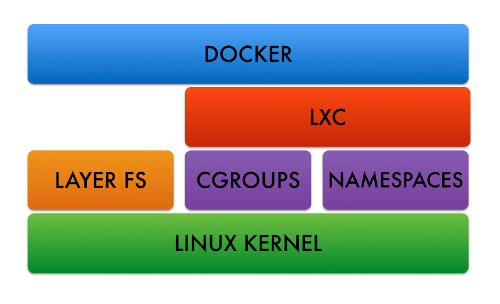
\includegraphics[scale=0.7]{pics/docker_arch.png}
	\caption{Wysokopoziomowe spojrzenie na architekturę systemu Docker}
	\label{docker_arch}
\end{figure}

Na rysunku \ref{docker_arch} przedstawiono stos technologiczny rozwiązania Docker. Na samym dole stosu znajduje się serwer, czyli fizyczna maszyna na której uruchomiony jest system operacyjny. Ten uruchomiony system będzie służył do uruchamiania kontenerów i to jego zasoby będą wydzielane dla poszczególnych kontenerów. Na systemie hoście należy zainstalować pakiet docker-engine. Umożliwi to nam uruchamianie kontenerów z przygotowanych wcześniej obrazów, w których będą znajdowały się faktyczne aplikacje oraz wszystkie potrzebne tym aplikacjom biblioteki. Zaleca się aby uruchamiać tylko jedną aplikację w danym kontenerze. Ułatwia to chociażby wyciąganie logów z wnętrza kontenera, oraz odpowiedniemu wyizolowaniu aplikacji, gdyż zasoby możemy podać tyko dla konkretnego kontenera a nie dla każdego procesu. Tabela \ref{docker_cli} ukazuje listę komend rozwiązania docker, wraz z krótkim opisem i przykładem użycia. Najważniejszymi z nich są \textit{run, stop, delete, ps, images, build oraz exec}. Pozwalają one przejść tzw. \textit{Container lifecycle}, czyli cykl życia kontenera – zbudowanie obrazu, uruchomienie go, wykonanie w nim jakiejś operacji oraz zatrzymanie a następnie usunięcie go.

\begin{table}[!htbp]
\caption{Ważniejsze polecenia w programie docker (dla wersji 1.13.1)}
\label{docker_cli}
\begin{tabular}{|p{3cm}|p{11cm}|}
  \hline
  \textbf{Polecenie} & \textbf{Opis oraz przykład}\\
  \hline
  docker attach & Podłączenie się do uruchomionego już kontenera, celem przechwycenia wyjścia z aplikacji uruchomionej w kontenerze. Kontener należy wskazać poprzez identyfikator lub nazwę (pole obowiązkowe). \newline docker attach world-community-grid \\
  \hline
  docker build & Zbudowanie kontenera w oparciu o podany plik dockerfile. Narzędzie do budowania obrazów odszuka obraz który ma być podstawą dla naszego obrazu, a następnie wykona na nim wszystkie sekwencje wypisane w pliku Dockerfile. Ostatecznie na dysku zostanie zapisany gotowy do użycia obraz. O ile nie podamy parametru –tag jedynym sposobem na dostęp do obrazu będzie odwołanie się poprzez nadane ID.
  \newline docker build . -t  world-community-grid \newline Zakładając, że w bierzącym katalogu znajduje się plik poprawny plik Dockerfile po uruchomieniu tej komendy zostanie on przetworzony. Zbudowany obraz otrzyma ID oraz zostanie otagowany jako  world-community-grid:latest \\
  \hline
  docker commit & Umożliwia stworzenie nowego obrazu w oparciu o już istniejący kontener lub obraz. \newline docker commit --change "ENV DEBUG true" c3f279d17e0a rsmitty/boinc \\
  \hline
  docker cp & Kopiuje pliki między kontenerem a maszyną hostem i odwrotnie \newline docker cp /tmp/foo.txt world-community-grid:/tmp \\
  \hline
  docker create & Tworzy kontener na zasadzie identycznej jak docker run, z tą różnicą że kontener nie jest jeszcze uruchomiony i jego uruchomienie należy wykonać oddzielnie za pomocą docker start \newline docker create -t -i fedora bash \\
  \hline
  docker exec & Wykonuje podane polecenie we wskazanym kontenerze. Odpowiednie flagi decydują o lokalizacji wyjścia z podanego polecenia. \newline docker exec -it  world-community-grid bash \newline Uruchomi basha w kontenerze w sposób interaktywny. \\
  \hline
  docker images & Wyświetlanie listy obrazów pobranych i gotowych do użycia w systemie. \newline docker images –all \newline Wyświetlenie listy wszystkich obrazów znajdujących się na maszynie. \\
  \hline docker inspect & Wyświetlenie bardzo szczegółowych informacji na temat obrazu lub kontenera. \newline docker inspect  world-community-grid \\
  \hline docker ps & Wyświetlenie listy uruchomionych kontenerów. \newline docker ps -a \newline Wyświetli listę wszystkich kontenerów w systemie, nawet tych, które są zatrzymane bądź skończyły pracę. \\
  \hline docker pull & Pobieranie ze zdalnego repozytorium obrazów wskazanego obrazu \newline docker pull rsmitty/boinc \\
  \hline docker push & Opublikowanie na zewnętrznym repozytorium wskazanego obrazu obecnego w systemie \newline docker push rsmitty/boinc \\
  \hline docker rm & Usunięcie kontenera o wskazanej nazwie/ID \newline docker rm  world-community-grid \\
  \hline docker run & Stworzenie i uruchomienie kontera o określonych parametrach. \newline \newline docker run --restart=always -d --name wcg -e "boincurl=www.worldcommunitygrid.org" -e "boinckey=1033877\_ca3e3556f2fcafbb8edc82447e16b58c" rsmitty/boinc \newline Utworzy kontener z obrazu rsmitty/boinc (a jeśli taki nie jest obecny na dysku to docker podejmie próbę pobrania go). Do kontenera zostaną przekazane dwie zmienne środowiskowe i zostanie nadana mu nazwa world-community-grid.  \\
  \hline
\end{tabular}
\end{table}

 Nie trudno zauważyć, że w problemie konteneryzacji najważniejsze są dwa zagadnienia, tj. obsługa cyklu życia kontenera oraz zarządzanie obrazami. Obrazy dockerowe są trzymane w repozytoriach obrazów (ang. docker registry) a zarządzanie nimi odbywa się w sposób podobny do klasycznych repozytoriów kodu. W centrum danych można uruchomić takie repozytorium i przechowywać na nim obrazy. Dzięki temu zabiegowi wystarczy tylko raz zbudować obraz (co przy złożonych obrazach zajmuje wiele czasu) i po jego przesłaniu (polecenie docker push) można taki obraz pobrać (polecenie docker pull) na pozostałych serwerach w centrum danych.

 Obrazy w dokerze opierają się na plikach Dockerfile. Są to pliki tekstowe, w których musi zostać uwzględniona notacja Dockera oraz przygotowane dla użytkownika dyrektywy. Najważniejsze z nich to \textit{FROM, RUN}, oraz \textit{CMD}:

\begin{itemize}
\item Dyrektywa \textit{FROM} pozwala na wskazanie jaki obraz ma być podstawą dla opisywanego właśnie obrazu. Ta dyrektywa powinna pojawiać się na samym początku pliku Dockerfile.
\item \textit{RUN} pozwala na wykonywanie poleceń. Narzędzie do budowania obrazów uruchomi każdą komendę i jej wynik zapisze do „mini” obrazu (warstwy). Przy zakończeniu budowania wszystkie warstwy zostaną złączone w jeden obraz. To podejście ma ogromną zaletę: przebudowywanie komend raz już wykonanych jest szybkie, gdyż po prostu zostanie użyta zbudowana wcześniej warstwa. Przykładowy stos warstw obrazu pokazany jest na rysunku (Rys. \ref{docker_layers}).
\begin{figure}[ht!]
	\centering
	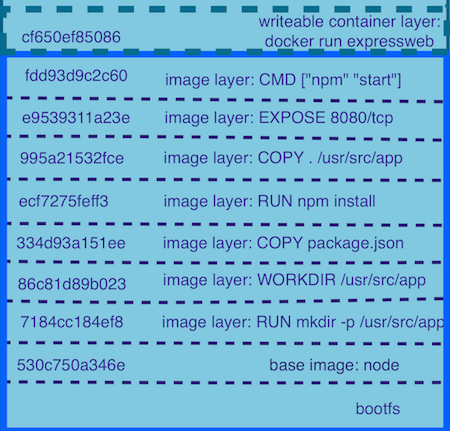
\includegraphics[scale=0.7]{pics/docker_layers.png}
	\caption{Lista warstw jakie składają się na obraz ‘expressweb’.}
	\label{docker_layers}
\end{figure}
\item \textit{CMD} określa komendę jaka zostanie uruchomiona przy starcie kontenera. Poprawne ustawienie tego polecenia jest kluczowe dla właściwego działania aplikacji. To właśnie logi tego polecenia będą znajdowały się na wyjściu polecenia docker logs.
\end{itemize}

W związku z tym, że nie każdy użytkownik ma zestawione swoje repozytorium firma docker uruchomiła swoje własne, które jest dostępne w Internecie. Prócz repozytorium obrazów jest dostępny też web serwis, który w przyjaznej firmie prezentuje wszystkie informacje. Produkt jest dostępny pod adresem https://hub.docker.com

\begin{figure}[!h]
	\centering
	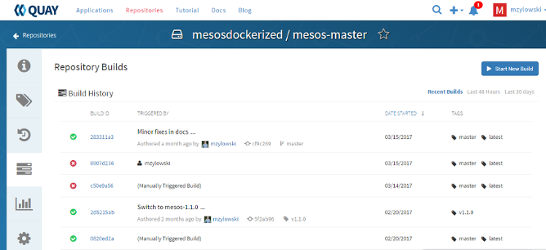
\includegraphics[scale=1]{pics/quay.png}
	\caption{Historia przebudowywania obrazu mesos-master napisanego na potrzeby tej pracy.}
	\label{quay_io}
\end{figure}

Ze względu na monopol dockera pojawił się projekt wspierający inne formaty obrazów. Mowa tutaj o repozytorium i web serwisie dostępnym pod adresem https://quay.io. Na rysunku \ref{quay_io} widoczny jest zrzut ekranu z serwisu quay.io.

TODO: W razie czego można opisać jeszcze: marketing dockera, nie trzymanie się standardów, problemy platformy, praktyczne zastosowania.

\subsection{Rozwiązanie konteneryzacyjne \textit{rkt}}

\begin{figure}[!h]
	\centering
	
\includegraphics[scale=1]{pics/rkt-horizontal-color.png}
	\caption{Logo projektu rkt}
	\label{rkt_logo}
\end{figure}

Rkt (Rys. \ref{rkt_logo}) jest produktem sponsorowanym przez firmę CoreOS i jest próbą wydarcia części rynku Dockerowi. Rkt jest aplikacją pozwalającą uruchamiać kontenery na systemach z rodziny Linux, a celem przyświecającym twórcom aplikacji było zaprojektowanie jej tak by:

\begin{itemize}
\item Bazowała na \textit{podach} - \textit{pod} to mechanizm pozwalający uruchamiać wiele kontenerów w jednym bycie. Ułatwia to łączenie aplikacji między sobą i ich organizowanie. Kontenery realizujące zadania ze sobą powiązane mogą być trzymane w jednym podzie, co dodatkowo oddziela je od innych zadań w systemie. Zadania w jednym podzie mogą interferować między sobą. Pod można rozumieć jako kolejną wartstę abstrakcji oddzielająca procesy uruchomione przez system operacyjny.
\item Zapewniała bezpieczeństwo bez żadnych dodatkowych konfiguracji - natywne wsparcie dla mechanizmu \textit{SELinux} oraz uruchamianie aplikacji w maszynach wirtualnych.
\item Integrowała się z innymi systemami związanymi z uruchamianiem zadań (\textit{systemd}, \textit{upstart}) oraz z orkiestratorami zadań na klastrach (\textit{Kubernetes}, \textit{Nomad}).
\item Wspierała i zachowywała standardy dotyczące konteneryzacji oraz współpracowała z istniejącymi formatami obrazów. Rkt potrafi uruchomić obraz w specyfikacji \textit{OCI} lub obraz zbudowany oprogramowaniem docker. Produkt wykorzystuje rozwiązania projektu \textit{Container Networking Interface}, który rozwiązuje problem sieci między uruchomionymi kontenerami.
\end{itemize}

\begin{figure}[!h]
	\centering
	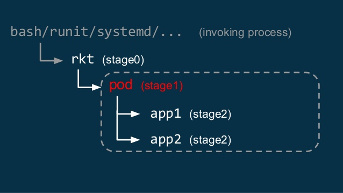
\includegraphics[scale=1]{pics/rkt-architecure.jpg}
	\caption{Architektura rozwiązania rkt}
	\label{rkt_arch}
\end{figure}

Rozwiązanie rkt bazuje na tak zwanych ang. \textit{stage}. Pozwalają one na wyraźne rozgraniczanie poszczególnych modułów systemów co umożliwia wprowadzenie warstwowej podmienialnej architektury całego rozwiązania. Na rysunku \ref{rkt_arch} przedstawiono architekturę tego rozwiązania (przy uruchomionym jednym podzie i dwóch kontenerach). I tak:

\begin{itemize}
\item stage0 - jest to poziom systemu operacyjnego i procesu samej aplikacji rkt.
\item stage1 - jest to poziom poda, swego rodzaju baza dla dalszego uruchamiania kontenerów. Stage1 to bardzo mocno okrojony system plików, który umożliwia uruchamianie prostych aplikacji i ploleceń systemu operacyjnego. W tym miejscu uwidacznia się jedna z największych sił rozwiązania rkt. Stage pierwszy może być podmieniany (jest tak naprawdę obrazem systemu plików). W zależności od wskazanego obrazu określimy sposób w jaki rkt będzie dokonywał izolowania uruchomionych później kontenerów. Aktualnie wraz z rozwiązaniem dostarczanych jest pięć obrazów, które mogą być tutaj wykorzystane (tabela \ref{rkt_flavors}).
\item stage2 - jest to poziom aplikacji uruchomionej w kontenerze. Wskazany obraz zostaje uruchomiony za pomocą odpowiedniego \textit{hypervizora}.
\end{itemize}

\begin{table}[!htbp]
\caption{Lista obrazów, które mogą być użyte jako stage1 w systemie konteneryzacji rkt}
\label{rkt_flavors}
\centering

\begin{tabular}{|p{3cm}|p{3cm}|p{8cm}|}
  \hline
  \textbf{Nazwa rozwiązania} & \textbf{Wykorzystywany mechanizm izolacji} & \textbf{Opis mechanizmu izolacji}\\
  \hline
  Fly & System plików i polecenie chroot & Ten mechanizm izolacji polega na skopiowaniu zawartości obrazu do innej lokalizacji a następnie wykonaniu tam polecenia chroot. W tym podejściu nie istnieje w zasadzie izolacja procesów uruchomionych w kontenerze. Będą one interferowały inne aplikacje uruchomione w systemie operacyjnym. Jedynym zystkiem z tej izolacji uniemożliwieniu użytkownikowi wyjście poza kontener (ucieczka do systemu gospodarza). \\
  \hline
  Rkt stage1 & systemd-nspawn, cgroups & Domyślny mechanizm izolacji stosowany w rkt. Zostanie wykorzystany jeśli parametr --stage1-name nie zostanie podany do polecenia uruchamiającego kontener. Jest to mechanizm analogiczny do już wcześniej opisanego sposobu izolacji wykorzystywanego w Dokerze. Podobnie jak w mechaniźmie \textit{Fly} zawartość obrazu jest rozpakowywana do lokalizacji w systemie operacyjnym a następnie polecenie chroot więzi użytkownika w odpowiednim katalogu. W tym rozwiązaniu jednak procesy kontenera są izolowane za pomocą mechanizm \textit{cgroup} (analogicznie jak w dokerze). \\
  \hline
  LKVM & Wirtualizacja KVM & To podejście jest kolejnym wyróżnikiem rkt. LKVM (\textit{lightweight} KVM) to niewielka aplikacja, która umożliwa uruchamianie maszyn wirtualnych wykorzystując sprzętowe technologie wirtualizacyjne. Dla procesorów AMD jest to technologia AMD-V, zaś dla procesorów rodziny intel Intel VT-x. Uruchomienie kontenera za pomocą programu LKVM to w zasadzie uruchomienie prostej maszyni wirtualnej. To podejście zapewnia wysoki poziom izolacji. \\
  \hline
  QEMU & Wirtualizacja KVM & Projekt LKVM w swoich założeniach miał być projektem lekkim, co wraz z rozwojem projektu rkt rodziło wiele problemów. Latem 2016 roku podjęto decyzje by zaimplementować konteneryzację wykorzystując technologię QEMU. QEMU jest rozwiązaniem bardzo rozbudowanym - umożliwia zarówno wykorzystanie emulacji sprzętowej jak i technologi KVM. Przez złożoność rozwiązania doszło do znaczącego spadku wydajności i wkrótce quemu zostało zastąpione pakietem quemu-lite. \\
  \hline
  XEN & Wirtualizacja XEN & Zewnętrzni klienci produktu rkt aby wypromować swoje rozwiązanie przygotowali stage1 oparty na wirtualizacji XEN. Na dzień pisania tej pracy projekt jest w fazie rozwojowej i nie jest używalny produkcyjnie. \\
  \hline
\end{tabular}
\end{table}


\newpage
%TODO
\section{Orkiestratory zadań}

\subsection{Apach Mesos}

Produkt \ref{mesos_logo} \textit{open source} przeznaczony do instalacji w centrum danych oferujący możliwość uruchamiania zadań na zadanych zasobach. Rozwijany początkowo na Uniwerystecie w Berkeley. Pierwsza prezentacja Mesosa miała miejsce w 2009 roku podczas konferencji \textit{HotCloud}. Projektem zainteresowała się fundacja Apache, która do dnia dzisiejszego zajmuje się rozwojem produktu. W Lipcu 2016 została wydana wersja 1.0 Mesosa (przeskok z wersji 0.26). Na ten krok zdecydowano się po zaimplementowaniu wielu dodatkowych funkcji, po dołączeniu do projektu firmy Mesosphera. Tak przygotowany produkt firma Mesosphera zaczęła rozprowadzać pod swoim logo jako kompleny produkt pozwalający osiągnąć wysoką utylizację centrum danych. Mowa tutaj o produkcie DC/OS \textit{Data Center Operating System}. 

\begin{figure}[!h]
	\centering
	
\includegraphics[scale=1]{pics/apache_mesos_logo.png}
	\caption{Logo projektu Apache Mesos}
	\label{mesos_logo}
\end{figure}

Mesos architektonicznie jest projektem, który zbiera zasoby ze wszystkich komputerów na których jest uruchomiony i przedstawia ją jako zunifikowaną pulę. Następnie pula ta może być użyta do uruchomienia zadań. Do zebranych zasobów należy się odwołać używając bądź implementując własny \textit{framework}. W tym miejscu uwidacznia się siła rozwiązania, ponieważ niewielkim wysiłkiem można zaprojektować swoje własne rozwiązanie, które będzie efektywnie rozdzielało zadania do wykonania. Umożliwia to specjalne programowe API, które wystawia Mesos.

Mesos początkowo wszystkie zadania uruchamiał jako kolejne procesy na wybranej do egzekucji maszynie. To podejście było bardzo prostą izolacją, która dopiero później była dalej rozwijana. Również procesy odpowiedzialne za działanie Mesosa były uruchamiane jako zwykłe procesy, tak więc zadanie uruchomione w Mesosie mogło w skrajnej sytuacji interferować nawet proces samego kontrolera klastra. Popoularność rozwiązania Docker sprawiła, że do Mesosa dodano możliwość uruchomienia skonteneryzowanych aplikacji. Dodatkowo zaleca się uruchomienie poszczególnych procesów dockera w osobnych kontenerach, w ten sposób wszystkie uruchomione zadania są od siebie izolowane i nie interferują procesów samego Mesosa.

Na dzień pisania tej pracy Mesos posiada tylko eksperymentalne wsparcie dla kontenerów \textit{appc}. Nie jest możliwe uruchamianie wielu kontenerów w jednym podzie, a samo wspracie dla rkt nie jest stabilne. Przyczyną tego stanu rzeczy jest niechęć firmy Mesosphera do wspierania produktu konkurencyjnego dla Dokera i prawdopodobnie tak długo jak rkt nie zdobędzie większej popularności, tak długo Mesos nie będzie posiadał produkcyjnego wsparcia dla wszystkich mechanizmów, które oferuje rkt.

Architektura Mesosa oraz istniejące na rynku \textit{frameworki} zostały opisane w kolejnym rozdziale tej pracy. 

\subsection{Kubernetes}

Kubernetes (rys. \ref{kube_logo}) - znacznie młodsza konkurencja rozwiązania Mesos (po raz pierwszy ogłoszony publicznie w połowie roku 2014). Sponsorowany i rozwijany jako wolne oprogramowanie przez korporację Google. Rozwiązanie od samego początku oparte było o kontenery Dockera. Nigdy nie powstała możliwość uruchamiania pojedyńczych procesów w systemie operacyjnym (tak jak w Mesosie). Kubernetes jako rozwiązanie młode często wprowadza zmiany architektoniczne i nowe możliwości. Jego niedojrzałość powoduje, że trzeba włożyć więcej pracy w aktualizacje klastra i zapewnienie stabilności. Przykładem zmiany, która doprowadziła do takich problemów może być mechanizm CRI \textit{Container Runtime Interface}. Ze względu na pojawiające się konkurencyjne do Dokera rozwiązania kontenerowe (rkt, OCI) w kubernetesie zaprojektowano mechanizm CRI. Jest to programowe API działające po specjalnie przygotowanej przez Google implementacji protokołu RPC - GRPC. Dany \textit{runtime} kontenerowy musi implementować to API by porozumiewać się z kubernetesem. Rozwiązania kontenerowe zaprojektowały swoje odzielne procesy, których celem była komunikacja po interfejsie CRI. Dla rkt jest to proces \textit{rktlet} a dla Dockera \textit{docker-shim}. Zainstalowanie wersji 1.6 wymagało również aktualizację konteneryzatora, a to wymagało wyłączenia bądź przemigrowania usług działających na danym komputerze w klastrze. Porównanie architektury kubernetesa 1.5 z 1.6 przedstawiono odpowiednie na rysunkach \ref{k8s_1_5} i \ref{k8s_1_6}.

\begin{figure}[!h]
	\centering
	
\includegraphics[scale=1]{pics/Kubernetes-logo.png}
	\caption{Logo projektu Kubernetes}
	\label{kube_logo}
\end{figure}

Architektonicznie \ref{k8s_1_6} kubernetes jest mocno złożoną aplikacją. Poszczególne elementy aplikacji zostały porozdzielane na osobne usługi a nie jak w przypadku Mesosa zamknięte niemal w dwóch usługach. Wyróżnić należy szczególnie proces \textit{kubelet}, który jest sercem całego rozwiązania. Każdy komputer na którym uruchomiony jest proces kubeleta należy do klastra kubernetesa. Jest to jedny proces, który należy uruchomić z poziomu systemd. Wszystkie inne potrzebne procesy zostaną uruchomione jako byty kubernetesa (jako kontenery). Sam kubelet również może być uruchomiony w kontenerze, co jest domyślnym ustawieniem gdy klaster jest instalowany z narzędzia Kargo. 

\begin{figure}[!h]
	\centering
	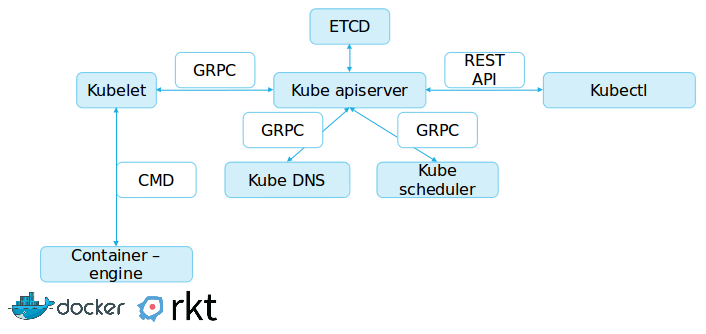
\includegraphics[scale=0.7]{pics/k8s_1_5.png}
	\caption{Architektura projektu Kubernetes w wersji 1.5}
	\label{k8s_1_5}
\end{figure}

\begin{figure}[!h]
	\centering
	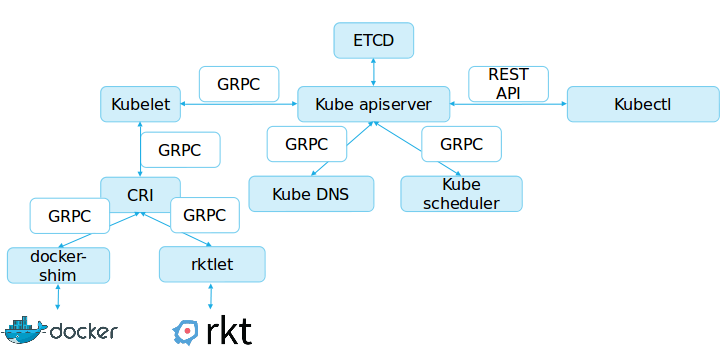
\includegraphics[scale=0.7]{pics/k8s_1_6.png}
	\caption{Architektura projektu Kubernetes w wersji 1.6. Widoczne są zmiany związne z dodaniem interfejsu CRI.}
	\label{k8s_1_6}
\end{figure}

Usługi w stosie architektonicznym kubernetesa komunikują się za pomocą protokołu GRPC. Wyjątkiem jest jedynie aplikacja \textit{kubectl}, która to komunikuje się z klastem za pomocą technologi REST API. \textit{Kubectl} jest programem pozwalającym komunikować się i zarządzać klastrem z poziomu konsoli \textit{bash}.

Prócz \textit{kubelet'a} i \textit{kubectl'a} do poprawnego działania klastra potrzebne są inne procesy:

\chapter{Nowy rozdział...}
\newpage

\listoffigures
\addcontentsline{toc}{chapter}{Spis rysunków}

\newpage

\listoftables
\addcontentsline{toc}{chapter}{Spis tabel}


\begin{thebibliography}{99}
\bibitem{ad1}Hamilton J., \textit{Internet-Scale Service Infrastructure Efficiency}, Symposium on Computer architecture, Jun. 2009.
\bibitem{ad2}Linthicum D., \textit{How to integrate with the cloud}, InfoWorld: Cloud Computing, April 27, 2011.
\bibitem{ad3}Kozyrakis Ch., \textit{Resource Efficient Computing for Warehouse-scale Datacenters}, 2013, Stanford University.
\bibitem{ad4}Carlson N., \textit{At Last — The Full Story Of How Facebook Was Founded}, Business Insider.
\bibitem{ad5}Data Center Knowledge blog [online].[dostęp 26.03.2017]. Dostępny w Internecie: http://www.datacenterknowledge.com/the-facebook-data-center-faq/
\bibitem{ad6}"Chip",\textit{Internet jest chmurą}, 03/2009, s. 38. Warszawa: Burda Communications sp. z o.o.. ISSN 1230-817X.
\bibitem{ad7}Trojnar D.,\textit{Wirtualizacja jako przyszłość sieci teleinformatycznych}, W: SECON 2010 – Materiały konferencyjne. Warszawa: WAT, 2010.
\bibitem{ad8}Levinson M., \textit{Software as a Service (SaaS) Definition and Solutions}.
\bibitem{ad9}Boniface, M., \textit{Platform-as-a-Service Architecture for Real-Time Quality of Service Management in Clouds}, 5th International Conference on Internet and Web Applications and Services (ICIW), Barcelona, Spain: IEEE, pp. 155–160, doi:10.1109/ICIW.2010.91
\bibitem{ad10}Mell P., Grence T., \textit{The NIST Definition of Cloud Computing (Technical report)}, MNational Institute of Standards and Technology: U.S. Department of Commerce. doi:10.6028/NIST.SP.800-145. Special publication 800-145.
\bibitem{ad11}Rouse M.,\textit{What is public cloud?}, Definition from Whatis.com.
\bibitem{ad12}Bernstein D., Ludvigson E., Sankar K., Diamond S., Morrow M., \textit{Blueprint for the Intercloud – Protocols and Formats for Cloud Computing Interoperability}, IEEE Computer Society: 328–336. doi:10.1109/ICIW.2009.55. ISBN 978-1-4244-3851-8.
\bibitem{ad13}Krause S.,\textit{The private vs public cloud debate: Which to deploy, and why consider hybrid?}, cloudcomputing news.
\bibitem{ad14}Freedman R., \textit{Cloud computing migration issues: What you need to know} [online].[dostęp 14.04.2017]. Dostępny w Internecie: http://www.techrepublic.com/blog/it-consultant/cloud-computing-migration-issues-what-you-need-to-know/.
\bibitem{ad15}Krasuski T., Łoś J., Szostakiewicz M.,\textit{Wstęp do wirtualizacji}, Uniwersytet Warszawski, 2005.
\begin{comment}
....
https://github.com/rkt/rkt/pull/2952
https://github.com/rkt/rkt/issues/3019#issuecomment-246637570
\end{comment}


\end{thebibliography}

\addcontentsline{toc}{chapter}{Bibliografia}

\end{document}
